\normaltrue \difficilefalse \tdifficilefalse
\correctionfalse
%\UPSTIidClasse{11} % 11 sup, 12 spé
%\newcommand{\UPSTIidClasse}{11}

\exer{Palettisation -- Stabilité$\star$ \label{C2:03:stab:62}}
%% CCP MP 2010
\setcounter{numques}{0}
\UPSTIcompetence[2]{C2-03}
\index{Compétence C2-03}
\index{Schéma-blocs}
\index{Stabilité}

\ifcorrection
\else
\textbf{Pas de corrigé pour cet exercice.}
\fi


\ifprof 
\else
Une boucle de position est représentée ci-dessous. On admet que :  
\begin{itemize}
\item $H(p)=\dfrac{\Omega_m(p)}{U_v(p)}=\dfrac{30}{1+\num{5e-3}p}$;
\item $K_r = \SI{4}{V.rad^{-1}}$ : gain du capteur de position;
\item $K_a$ : gain de l’adaptateur du signal de consigne $\alpha_e(t)$; 
\item $N=200$ : rapport de transmission du réducteur (la réduction est donc de $1/N$).
\item le signal de consigne $\alpha_e(t)$ est exprimé en degré ; 
\item le correcteur $C(p)$ est à action proportionnelle de gain réglable $K_c$. 
\end{itemize}


\begin{center}
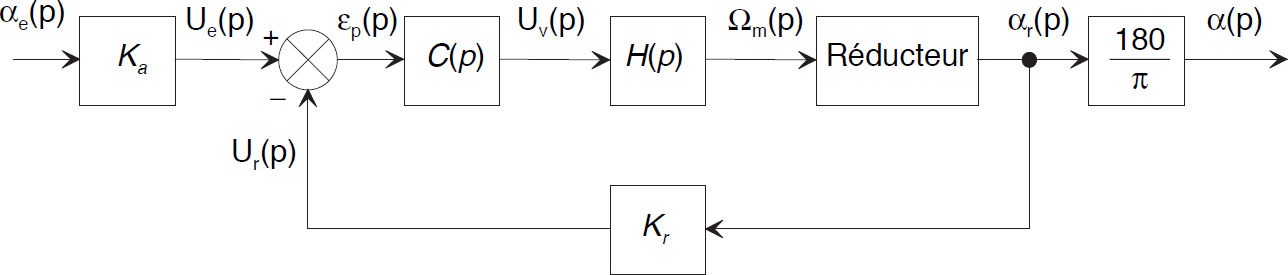
\includegraphics[width=.9\linewidth]{62_01}
\end{center}
 \fi
 
 
 On montre que la fonction de transfert du réducteur est $R(p)=\dfrac{\alpha_r(p)}{\Omega_m(p)}=\dfrac{1}{Np}$, que  $k_a=\dfrac{\pi}{180}k_r$ et que la FTBO est donnée par $T(p)=\dfrac{k_{BO}}{p\left(1+\tau_m p\right)}$ ($k_{BO}=\dfrac{k_c k_m k_r}{N}$).
 
 
 On souhaite une marge de phase de 45\degres.
\question{Déterminer la valeur de $K_{BO}$ permettant de satisfaire cette condition.}
\ifprof
\else 
\fi

\question{En déduire la valeur du gain $K_c$ du correcteur. }
\ifprof
\else 
\fi

\question{Déterminer l’écart de position.}
\ifprof
\else 
\fi

 

\ifprof
\else

\noindent\footnotesize
\fbox{\parbox{.9\linewidth}{
Éléments de corrigé : 
\begin{enumerate}
  \item $k_{BO}=\sqrt{2}{\tau_m}$.
    \item $k_c=\dfrac{\sqrt{2}N}{\tau_m k_m k_r} = 471,1$.
    \item $\varepsilon_s=0$.
\end{enumerate}}}
\normalsize

\begin{flushright}
\footnotesize{Corrigé  voir \ref{C2:03:stab:62}.}
\end{flushright}%
\fi